% Three active slides; the optional accuracy slide remains commented out below.
% Editable vector figures. Findings are recorded tests from
% 1--3 October 2026; full evidence/file map: README_PROJECT_EXPLANATIONS.md.
% Self-contained: no external images, data files or project files are required.
\documentclass[aspectratio=169,11pt]{beamer}
\usepackage[T1]{fontenc}
\usepackage{lmodern}
\usepackage{booktabs,tabularx,tikz,graphicx}
\usetikzlibrary{arrows.meta,positioning,shapes.geometric}
\geometry{paperwidth=216mm,paperheight=121.5mm}
\definecolor{ink}{HTML}{16324F}
\definecolor{accent}{HTML}{087F8C}
\definecolor{muted}{HTML}{597081}
\setbeamercolor{normal text}{fg=ink,bg=white}
\setbeamercolor{frametitle}{fg=ink}
\setbeamercolor{structure}{fg=accent}
\setbeamertemplate{navigation symbols}{}
\setbeamertemplate{headline}{}
\setbeamertemplate{footline}{%
  \hfill\insertframenumber/\inserttotalframenumber\hspace{5mm}\vspace{3mm}}
\setbeamersize{text margin left=7mm,text margin right=7mm}
\setbeamerfont{frametitle}{size={\fontsize{21}{25}\selectfont},series=\bfseries}
\setlength{\tabcolsep}{4pt}
\renewcommand{\arraystretch}{1.12}
\newcommand{\file}[1]{{\ttfamily\detokenize{#1}}}
\newcolumntype{Y}{>{\raggedright\arraybackslash}X}

% Diagram labels and the optional accuracy chart's recorded values.
\newcommand{\migrationOld}{Ubuntu 20.04\\ROS Foxy / TensorRT 8}
\newcommand{\migrationWork}{Update APIs\\Check sizes / reuse buffers}
\newcommand{\migrationNew}{Ubuntu 24.04\\ROS Jazzy / TensorRT 10}
\newcommand{\migrationCaption}{Same pretrained ONNX; no retraining.}
\newcommand{\flowInput}{LiDAR driver or rosbag player}
\newcommand{\flowCallback}{CPU: ROS callback}
\newcommand{\flowCpuIn}{CPU: validate and pack XYZI}
\newcommand{\flowGpu}{GPU: PointPillars engine}
\newcommand{\flowCpuOut}{CPU: validate boxes and run NMS}
\newcommand{\flowMessage}{CPU: construct Detection3DArray}
\newcommand{\flowView}{RViz or another consumer}
\newcommand{\flowCaption}{TensorRT's CPU API schedules GPU work. ROS runs on the CPU.}
\newcommand{\flowInputTransfer}{ROS /point\_cloud}
\newcommand{\flowToGpu}{CUDA: copy points and count\\to GPU}
\newcommand{\flowFromGpu}{CUDA: copy candidate boxes\\to CPU}
\newcommand{\flowOutputTransfer}{ROS /bbox}
\newcommand{\flowDirect}{ROS point-cloud topic}
\newcommand{\engineDownload}{Docker build: download ONNX\\and verify its checksum}
\newcommand{\engineStartup}{Container startup:\\check GPU, model and cache}
\newcommand{\engineDecision}{Matching engine\\in cache?}
\newcommand{\engineReuse}{Reuse existing\\engine}
\newcommand{\engineBuild}{trtexec: build engine\\from ONNX}
\newcommand{\engineStored}{Engine in persistent storage}
\newcommand{\engineLoad}{ros2 run: load engine once}
\newcommand{\engineInfer}{Reuse engine for every cloud}
% BEV AP_R40 percentages: config/kitti_accuracy_inventory.json, test/moderate.
\newcommand{\chartCar}{5.75160104747}
\newcommand{\chartPedestrian}{0}
\newcommand{\chartCyclist}{0.0257731958763}
\newcommand{\chartTitle}{BEV AP (R40, \%)}
\newcommand{\chartCaption}{16 moderate test frames; small diagnostic set.}
\newcommand{\chartSource}{Source: config/kitti_accuracy_inventory.json}

\newcommand{\migrationfigure}{%
  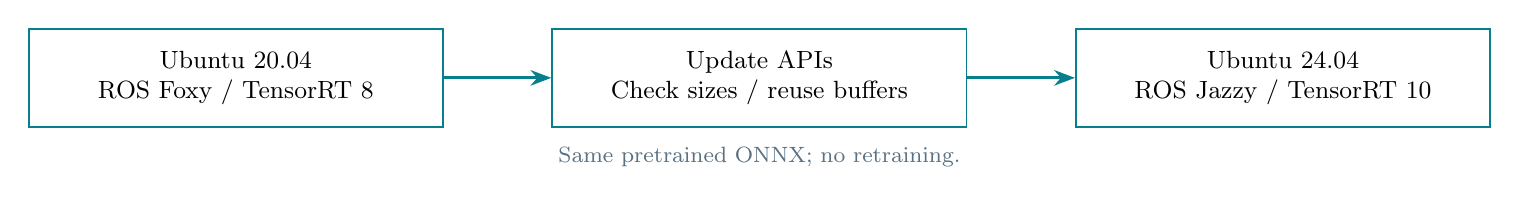
\begin{tikzpicture}[x=1cm,y=1cm,font=\small,>=Stealth,
    stage/.style={draw=accent,line width=.7pt,align=center,
                  minimum height=1.25cm,text width=5.05cm,inner sep=3pt}]
    \node[stage] (old) at (0,0) {\migrationOld};
    \node[stage] (work) at (6.65,0) {\migrationWork};
    \node[stage] (new) at (13.3,0) {\migrationNew};
    \draw[->,accent,line width=1pt] (old.east) -- (work.west);
    \draw[->,accent,line width=1pt] (work.east) -- (new.west);
    \node[font=\footnotesize,text=muted] at (6.65,-1.0) {\migrationCaption};
  \end{tikzpicture}%
}

\newcommand{\runtimefigure}{%
  % Native TikZ version of the user's top-to-bottom Mermaid flowchart.
  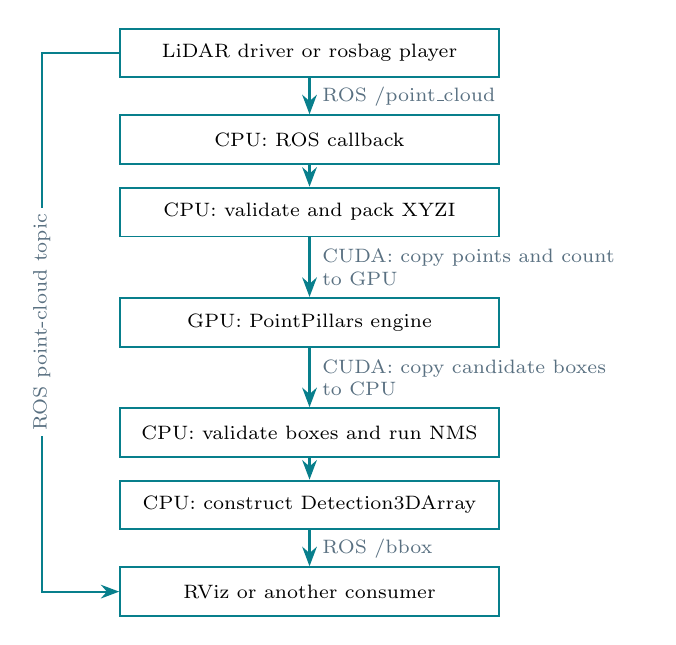
\begin{tikzpicture}[x=1cm,y=1cm,font=\scriptsize,>=Stealth,
    stage/.style={draw=accent,line width=.7pt,align=center,
                  minimum height=.62cm,text width=4.6cm,inner sep=3pt},
    transfer/.style={font=\scriptsize,text=muted,align=left,
                     anchor=west,text width=4.1cm,inner sep=1pt}]
    \node[stage] (input) at (0,0) {\flowInput};
    \node[stage] (callback) at (0,-1.10) {\flowCallback};
    \node[stage] (cpuin) at (0,-2.02) {\flowCpuIn};
    \node[stage] (gpu) at (0,-3.42) {\flowGpu};
    \node[stage] (cpuout) at (0,-4.82) {\flowCpuOut};
    \node[stage] (message) at (0,-5.74) {\flowMessage};
    \node[stage] (view) at (0,-6.84) {\flowView};
    \draw[->,accent,line width=.9pt] (input.south) -- (callback.north);
    \draw[->,accent,line width=.9pt] (callback.south) -- (cpuin.north);
    \draw[->,accent,line width=.9pt] (cpuin.south) -- (gpu.north);
    \draw[->,accent,line width=.9pt] (gpu.south) -- (cpuout.north);
    \draw[->,accent,line width=.9pt] (cpuout.south) -- (message.north);
    \draw[->,accent,line width=.9pt] (message.south) -- (view.north);
    \node[transfer] at (.12,-.55) {\flowInputTransfer};
    \node[transfer] at (.12,-2.72) {\flowToGpu};
    \node[transfer] at (.12,-4.12) {\flowFromGpu};
    \node[transfer] at (.12,-6.29) {\flowOutputTransfer};
    % Direct source-to-consumer edge, independent of the detection pipeline.
    \draw[->,accent,line width=.8pt] (input.west) -- (-3.4,0)
      -- (-3.4,-6.84) -- (view.west);
    \node[rotate=90,font=\scriptsize,fill=white,text=muted,inner sep=2pt]
      at (-3.4,-3.42) {\flowDirect};
  \end{tikzpicture}%
}

\newcommand{\enginefigure}{%
  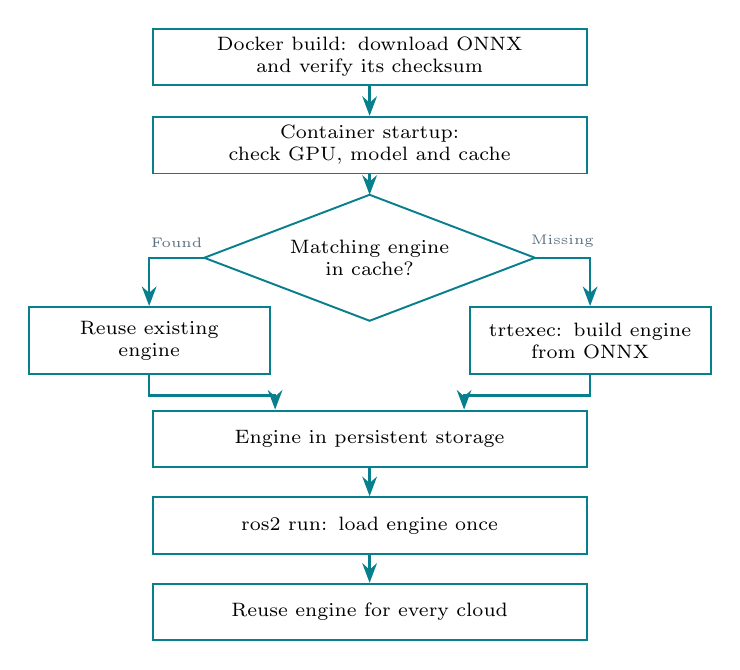
\begin{tikzpicture}[x=1cm,y=1cm,font=\scriptsize,>=Stealth,
    stage/.style={draw=accent,line width=.7pt,align=center,
                  minimum height=.72cm,text width=5.3cm,inner sep=3pt},
    branch/.style={stage,text width=2.85cm,minimum height=.85cm},
    link/.style={->,accent,line width=.9pt}]
    \node[stage] (download) at (0,0) {\engineDownload};
    \node[stage] (startup) at (0,-1.12) {\engineStartup};
    % Fixed diamond bounds keep the decision clear of the surrounding boxes.
    \draw[accent,line width=.7pt] (0,-1.75) -- (2.1,-2.55)
      -- (0,-3.35) -- (-2.1,-2.55) -- cycle;
    \node[align=center,text width=2.2cm,inner sep=1pt]
      at (0,-2.55) {\engineDecision};
    \coordinate (cacheNorth) at (0,-1.75);
    \coordinate (cacheWest) at (-2.1,-2.55);
    \coordinate (cacheEast) at (2.1,-2.55);
    \node[branch] (reuse) at (-2.8,-3.60) {\engineReuse};
    \node[branch] (build) at (2.8,-3.60) {\engineBuild};
    \node[stage] (stored) at (0,-4.85) {\engineStored};
    \node[stage] (load) at (0,-5.95) {\engineLoad};
    \node[stage] (infer) at (0,-7.05) {\engineInfer};
    \draw[link] (download.south) -- (startup.north);
    \draw[link] (startup.south) -- (cacheNorth);
    \draw[link] (cacheWest) -|
      node[pos=.25,above,font=\tiny,text=muted] {Found} (reuse.north);
    \draw[link] (cacheEast) -|
      node[pos=.25,above,font=\tiny,text=muted] {Missing} (build.north);
    \draw[link] (reuse.south) -- (-2.8,-4.3)
      -| ([xshift=-1.2cm]stored.north);
    \draw[link] (build.south) -- (2.8,-4.3)
      -| ([xshift=1.2cm]stored.north);
    \draw[link] (stored.south) -- (load.north);
    \draw[link] (load.south) -- (infer.north);
  \end{tikzpicture}%
}

\newcommand{\accuracyfigure}{%
  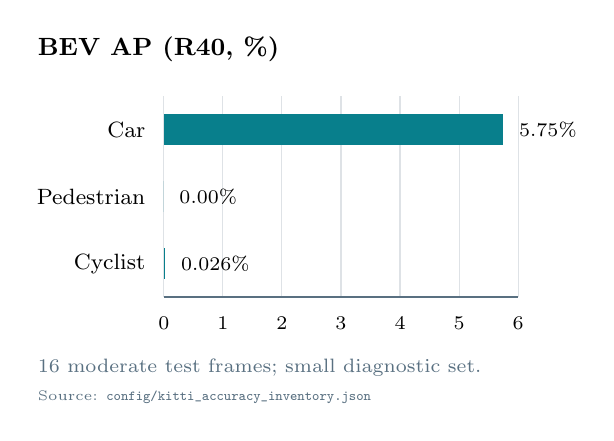
\begin{tikzpicture}[x=.75cm,y=.85cm,font=\footnotesize]
    \node[anchor=west,font=\small\bfseries] at (-2.3,4.2) {\chartTitle};
    \foreach \tick in {0,1,2,3,4,5,6} {
      \draw[muted!20] (\tick,.5) -- (\tick,3.5);
      \node[anchor=north,font=\scriptsize] at (\tick,.35) {\tick};
    }
    \draw[muted] (0,.5) -- (6,.5);
    % Do not use \value as a loop variable: LaTeX uses it for counters.
    \foreach \barCategory/\barScore/\barRow in
      {Car/\chartCar/3,Pedestrian/\chartPedestrian/2,Cyclist/\chartCyclist/1} {
      \node[anchor=east] at (-.15,\barRow) {\barCategory};
      \fill[accent] (0,{\barRow-.23}) rectangle ({\barScore},{\barRow+.23});
    }
    \node[anchor=west,font=\scriptsize] at (\chartCar+.10,3) {5.75\%};
    \node[anchor=west,font=\scriptsize] at (.10,2) {0.00\%};
    \node[anchor=west,font=\scriptsize] at (\chartCyclist+.10,1) {0.026\%};
    \node[anchor=west,font=\scriptsize,text=muted] at (-2.3,-.55) {\chartCaption};
    \node[anchor=west,font=\tiny,text=muted] at (-2.3,-1.0)
      {Source: \file{config/kitti_accuracy_inventory.json}};
  \end{tikzpicture}%
}

\title{PointPillars project migration}
\date{5 October 2026}
\begin{document}

\begin{frame}[t]{Why we updated the original code}
\small\raggedright
\textbf{Project purpose:} This project uses PointPillars to detect vehicles,
pedestrians and cyclists in LiDAR point clouds, then publishes their 3D boxes
through ROS 2 for visualization and use by other applications.

\smallskip
\centering\resizebox{.96\linewidth}{!}{\migrationfigure}\par
\raggedright
\small
Old ROS fields and TensorRT APIs did not fit the new stack. We also needed
checked data sizes, reliable cleanup and fewer GPU allocations.

\medskip
\begingroup\footnotesize
\begin{tabularx}{\linewidth}{@{}p{0.39\linewidth}Y@{}}
\toprule
\textbf{Main files we changed or added} & \textbf{What the change gives us} \\
\midrule
\file{CMakeLists.txt},\newline \file{package.xml} & C++17, explicit dependencies and CPU tests without a GPU. \\
\file{pp_inference_node.cpp},\newline \file{pointcloud_adapter.cpp} & Jazzy messages and checks before accepting a cloud. \\
\file{pointpillar.cpp},\newline \file{pointpillar.h} & TensorRT 10 named tensors, checked results and persistent runtime. \\
\file{cuda_resources.hpp},\newline \file{output_contract.hpp} & Reused GPU buffers, automatic cleanup and valid output counts. \\
\file{postprocess.cpp},\newline \file{postprocess.h} & Tested rotated box overlap and duplicate removal (NMS). \\
\bottomrule
\end{tabularx}
\endgroup

\end{frame}

\begin{frame}[t]{What the project supports today}
\begin{columns}[T,onlytextwidth]
\begin{column}{0.47\textwidth}
\centering
% Bound the vertical diagram so it leaves room for the title and footer.
\resizebox{!}{75mm}{\runtimefigure}
\end{column}
\begin{column}{0.50\textwidth}
\small\raggedright
\textbf{During inference}

\flowCaption

\medskip
\textbf{CPU responsibility}

Check and pack XYZI points. Validate returned boxes, remove duplicates with NMS,
and publish detections with the cloud's timestamp and coordinate frame.

\medskip
\textbf{GPU responsibility}

Group points into pillars, run the PointPillars network and decode candidate boxes.

\medskip
\textbf{Recorded checks}

CPU/ROS tests, 10 synthetic GPU frames, engine-cache reuse and 25 bag frames
in Docker plus 25 through host transport, with RViz.

\medskip
\textbf{Run settings}

\file{deploy.sh} and \file{node.yaml}: build/run command and settings.
The host provides the NVIDIA driver and Docker GPU access.

\medskip
\textbf{Tested:} Ubuntu 24.04, Linux x86-64, RTX 4060 Laptop.
\end{column}
\end{columns}

% \medskip
% \textbf{Still pending:} a background worker, configurable sensor QoS and sustained
% benchmarks. Today the callback is synchronous; the reliable queue is 700.
\end{frame}

\begin{frame}[t]{From ONNX to a running ROS node}
\begin{columns}[T,onlytextwidth]
\begin{column}{0.49\textwidth}
\centering
\resizebox{!}{76mm}{\enginefigure}
\end{column}
\begin{column}{0.48\textwidth}
\small\raggedright
\textbf{Two files, two jobs}

\file{.onnx}: trained network and weights, read by the builder.
\file{.engine}: GPU execution plan, read by the ROS node. No retraining.

\medskip
\textbf{Where they are stored}

Inside the container:\\
ONNX: \file{/opt/models/pointpillars.onnx}\\
Engine: \file{/var/lib/pp_infer/<key>.engine}\\
Default persistent volume: \file{pp-engines}.

\medskip
\textbf{When an engine is built}

First startup uses \file{trtexec} to build an FP32 engine for the selected GPU.
Later starts reuse a matching engine. The cache identity includes the model,
GPU, driver and build settings.

\medskip
\textbf{What ROS loads}

\file{engine_path} selects the engine. TensorRT loads it once into memory and
prepares GPU buffers. Each cloud reuses it.

\medskip
\textbf{Keep the ONNX in the image:} startup still checks its checksum.
Direct \file{ros2 run} requires an already prepared engine.
\end{column}
\end{columns}
\end{frame}

% \begin{frame}[t]{How we tested the code and what remains}
% \begin{columns}[T,onlytextwidth]
% \begin{column}{0.45\textwidth}
% \accuracyfigure
% \end{column}
% \begin{column}{0.52\textwidth}
% \footnotesize
% \begin{tabularx}{\textwidth}{@{}p{0.25\textwidth}X@{}}
% \toprule
% \textbf{Test layer} & \textbf{Recorded on 1--3 October 2026} \\
% \midrule
% CPU / ROS & 15 geometry cases; 2,000 random checks; 11 clouds; 2 parameter cases. \\
% GPU / Docker & 10 synthetic frames; plugins, bounds, empty inputs and engine/cache; 4 build tests. \\
% Real data & 25 bag frames in Docker + 25 through host transport; RViz rendered both. \\
% Reference & 32 labeled frames; 192 TRT8/TRT10 runs; identical-candidate NMS matched NVIDIA. \\
% \bottomrule
% \end{tabularx}
% \end{column}
% \end{columns}

% \medskip
% \small
% \textbf{The pipeline runs, but accuracy acceptance remains open.} The 16 moderate
% test frames had zero 3D true positives. Twelve matched test cars had a median
% upward center error of about 1.53 m.

% \medskip
% Repeated predictions vary; 12 of 32 clouds exceed the 10,000-pillar limit.
% Two capped-input controls improved repeatability. They did not prove the root cause.

% \medskip
% \textbf{Next:} model/input parity and bounded voxelization; broader GPU memory/failure
% checks. Evidence: \file{tests/}, \file{config/}, and the explanation README.
% \end{frame}

\end{document}
